\documentclass{article}
\usepackage{graphicx} % Required for inserting images
\usepackage[italian]{babel}
\usepackage{amsmath}
\usepackage[hidelinks]{hyperref}
\usepackage{amssymb}
\usepackage{algorithm}
\usepackage{algpseudocode}

\title{Introduzione agli algoritmi}
\author{Leonardo Ganzaroli}
\date{}

\begin{document}

\maketitle

\addcontentsline{toc}{section}{\protect\numberline{}Introduzione}

\tableofcontents

\newpage

\hypersetup{allcolors=black}

\section*{Introduzione}

Questi appunti sono derivanti principalmente dalle dispense del corso di \textit{Introduzione agli algoritmi} che ho svolto durante la laurea Triennale di informatica all'università "La Sapienza".

\newpage

\section{Nozioni di base}

\subsection{Alcune definizioni}

\textbf{Definizione} L'informatica è la scienza che consente di ordinare, trattare e trasmettere l’informazione attraverso l’elaborazione elettronica.\newline

\noindent Una definizione alternativa è \textit{L’informatica è la scienza degli algoritmi che descrivono e trasformano l’informazione: la loro teoria, analisi,
progetto, efficienza, realizzazione e applicazione}.\newline

\noindent \textbf{Definizione} Una struttura dati è un metodo per organizzare dati che prescinde dai dati stessi.\newline

\noindent\textbf{Definizione} Un algoritmo è una sequenza di comandi elementari ed
univoci che terminano in un tempo finito ed operano su
strutture dati.\newline

\noindent \textbf{Definizione} L'efficienza di un algoritmo è la quantificazione delle sue esigenze in termini di spazio e tempo.\newline

\noindent \textbf{Definizione} Il problem solving è un’attività atta a raggiungere una soluzione partendo da una situazione iniziale, in questo contesto è limitata ai problemi computazionali.\newline

\noindent \textbf{Definizione} Un problema computazionale è un problema che richiede di descrivere in modo automatico la relazione tra un insieme di valori di input e un insieme di valori di output.\newline

\noindent \textbf{Definizione} Un algoritmo si dice corretto se per ogni istanza di un certo problema esso termina producendo sempre l'output corretto.\newline

\newpage

\subsection{Modello del calcolatore}

Per poter calcolare i vari costi di un algoritmo è necessario usare un modello astratto di calcolatore, si può modellare con 4 elementi:
\begin{itemize}
    \item Processore
    \item Memoria centrale
    \item Memoria secondaria
    \item Dispositivi I/O
\end{itemize}

\begin{figure}[ht]
    \centering
    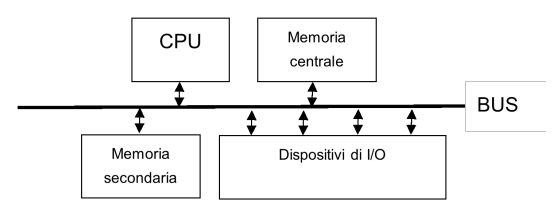
\includegraphics[width=0.75\linewidth]{Mod_calc.png}
    \caption{Connessione tra gli elementi}
    \label{fig:enter-label}
\end{figure}

\subsubsection{Memoria centrale/primaria} 

In questo caso ci si concentra sulla RAM (Random access memory) che può essere vista come una lunga sequenza di componenti elementari detti bit che possono assumere solo i valori 0 e 1.\newline

\noindent\textbf{Definizione} Un gruppo di 8 bits è detto byte.\newline

\noindent\textbf{Definizione} Un registro/parola di memoria è un aggregato di bytes, nei calcolatori moderni sono normalmente 4 o 8.\newline

\noindent Inoltre:
\begin{itemize}
    \item Il processore può operare su un registro (sia in lettura che scrittura) in una sola operazione
    \item Ogni parola ha un indirizzo 
    \item Il tempo per svolgere un'operazione è lo stesso indipendentemente dall'indirizzo
    \item Un indirizzo è un numero intero\newline
\end{itemize}

\noindent\textbf{Definizione} Lo spazio di indirizzamento è il numero di bit usati per rappresentare gli indirizzi.

\subsubsection{Memoria secondaria} 

La memoria secondaria ha le seguenti caratteristiche:
\begin{itemize}
    \item Conserva il contenuto
    \item È più lenta di quella centrale
    \item È più grande di quella centrale
    \item È più economica di quella centrale
\end{itemize}

\subsubsection{Random Access Machine}

Questo modello teorico astratto è caratterizzato da una memoria ad accesso casuale, un solo processore ed un insieme di istruzioni eseguite in tempo costante che permettono di fare:
\begin{itemize}
    \item I/O
    \item Operazioni aritmetiche
    \item Accesso e modifica del contenuto della memoria
    \item Salti
\end{itemize}

\subsection{Criterio della misura}

\textbf{Definizione} Il costo computazionale di un algoritmo è il suo tempo di esecuzione e/o le sue necessità in termini di memoria.

\paragraph{Costo uniforme}(Quello usato)\newline

\noindent Si parla di costo uniforme se si assume che
il costo di esecuzione dipende dalla dimensione degli operandi, ogni operazione è un singolo passo con costo 1.

\paragraph{Costo logaritmico}$\ $\newline

\noindent Si parla di costo logaritmico se si assume che il costo delle operazioni elementari è in funzione della dimensione degli operandi ($n\rightarrow \log n$).

\newpage

\section{Algoritmi}

\subsection{Notazione asintotica}

\textbf{Definizione} Per efficienza asintotica degli algoritmi si intende la valutazione del loro costo quando l'input è sufficientemente grande.\newline

\noindent\textbf{Definizione} Date $f(n),g(n)\geq 0$. Si dice che $f(n)$ è un $O(g(n))$ se:

$$\exists c,n_0\ |\ \forall\ n\geq n_0\ \ 0\leq f(n)\leq c*g(n)$$\newline

\begin{figure}[ht]
    \centering
    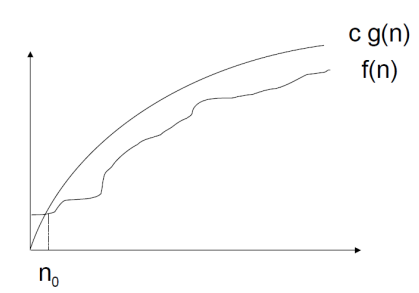
\includegraphics[width=0.6\linewidth]{O.png}
    \label{fig:O}
\end{figure}

\noindent\textbf{Definizione} Date $f(n),g(n)\geq 0$. Si dice che $f(n)$ è un $\Omega(g(n))$ se:

$$\exists c,n_0\ |\ \forall\ n\geq n_0\ \ f(n)\geq c*g(n)$$\newline

\begin{figure}[ht]
    \centering
    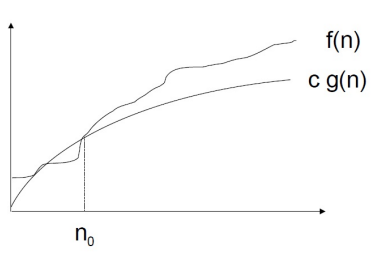
\includegraphics[width=0.6\linewidth]{omega.png}
    \label{fig:omega}
\end{figure}

\newpage

\noindent\textbf{Definizione} Date $f(n),g(n)\geq 0$. Si dice che $f(n)$ è un $\Theta(g(n))$ se:

$$\exists c_1,c_2,n_0\ |\ \forall\ n\geq n_0\ \ c_1*g(n)\leq f(n)\leq c_2*g(n)$$\newline

\begin{figure}[ht]
    \centering
    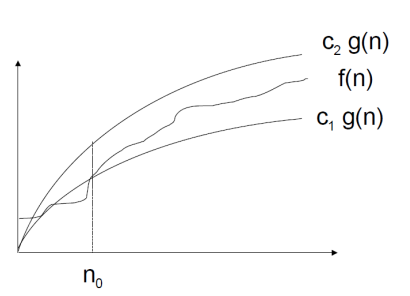
\includegraphics[width=0.6\linewidth]{theta.png}
    \label{fig:theta}
\end{figure}

\noindent Quindi $f(n)$ deve essere sia $\Omega(g(n))$ che $O(g(n))$.

\noindent\rule{\textwidth}{0.5pt}\newline

\noindent Esempio:\newline

\begin{itemize}
    \item $n^2+4n$ è $O(n^2)$

    Infatti se $c\geq5$ si ha che $\forall \ n \ \ n^2+4n\leq c*n^2$.

    \item $2n^2+3$ è $\Omega(n^2)$

    Infatti se $c\leq2$ si ha che $\forall \ n \ \ 2n^2+3\geq c*n^2$.

    \item $(n+10)^3$ è $\Theta(n^3)$

    Per $\Omega$ basta prendere $n_0=c=1$, per $O$ invece $n_0=10,c=8$.
    
\end{itemize}

\noindent\rule{\textwidth}{0.5pt}\newline

\paragraph{Calcolo alternativo} $\ $\newline

\noindent Un altro modo per determinare la notazione di una funzione è tramite i limiti, infatti si può usare il risultato di $\lim_{n\rightarrow\infty}\frac{f(n)}{g(n)}$:
\begin{itemize}
    \item $>0\rightarrow f(n)=\Theta(g(n))$
    \item $=\infty\rightarrow f(n)=\Omega(g(n))$
    \item $=0\rightarrow f(n)=O(g(n))$
\end{itemize}

\subsubsection{Algebra}

Si possono seguire delle semplici regole che permettono di semplificare il calcolo del costo computazionale:
\begin{itemize}
    \item Costanti moltiplicative

        $\forall\ k>0,f(n)\geq0$:
        \begin{itemize}
            \item Se $f(n)$ è $O(g(n))$ allora $k*f(n)$ è $O(g(n))$

           \item Se $f(n)$ è $\Omega(g(n))$ allora $k*f(n)$ è $\Omega(g(n))$

            \item Se $f(n)$ è $\Theta(g(n))$ allora $k*f(n)$ è $\Theta(g(n))$
                        
        \end{itemize}
    
    \item Commutatività somma

        $\forall\ f(n),d(n)>0$:
        \begin{itemize}
            \item Se $f(n)$ è $O(g(n))$ e $d(n)$ è $O(h(n))$ allora $f(n)+d(n)=O(g(n)+h(n))=O(max(g(n),h(n)))$

            \item Se $f(n)$ è $\Omega(g(n))$ e $d(n)$ è $\Omega(h(n))$ allora $f(n)+d(n)=\Omega(g(n)+h(n))=\Omega(max(g(n),h(n)))$

            \item Se $f(n)$ è $\Theta(g(n))$ e $d(n)$ è $\Theta(h(n))$ allora $f(n)+d(n)=\Theta(g(n)+h(n))=\Theta(max(g(n),h(n)))$
            
        \end{itemize}
    
    \item Commutatività prodotto

        $\forall\ f(n),d(n)>0$:
        \begin{itemize}
            \item Se $f(n)$ è $O(g(n))$ e $d(n)$ è $O(h(n))$ allora $f(n)*d(n)=O(g(n)*h(n))$

            \item Se $f(n)$ è $\Omega(g(n))$ e $d(n)$ è $\Omega(h(n))$ allora $f(n)*d(n)=\Omega(g(n)*h(n))$

            \item Se $f(n)$ è $\Theta(g(n))$ e $d(n)$ è $\Theta(h(n))$ allora $f(n)*d(n)=\Theta(g(n)*h(n))$
            
        \end{itemize}
    
\end{itemize}

\noindent\rule{\textwidth}{0.5pt}\newline

\noindent Esempio:

$$3n2^n+4n^4=\Theta(n)\Theta(2^n)+\Theta(n^4)=\Theta(n2^n)+\Theta(n^4)=\Theta(n2^n)$$

\vspace{-5pt}

\noindent\rule{\textwidth}{0.5pt}\newline

\vspace{-15pt}

\subsection{Valutazione del costo}

\textbf{Definizione} Lo pseudocodice è un linguaggio di programmazione informale, esso ha le seguenti caratteristiche:
\begin{itemize}
    \item Contiene tutti i costrutti di controllo classici
    \item Usa il linguaggio naturale per specificare le operazioni
    \item Ignora la gestione degli errori\newline
\end{itemize}

\noindent Alcune regole:
\begin{itemize}
    \item Le istruzioni elementari hanno costo $\Theta(1)$
    \item L'istruzione \textit{if} ha costo pari alla somma di:
    \begin{itemize}
        \item Costo della verifica della condizione
        \item Massimo costo dei due rami
        \end{itemize}
        
    \item I cicli hanno costo pari alla somma di:
        \begin{itemize}
        \item Costo della verifica della condizione
        \item Somma dei costi massimi di ogni iterazione
        \end{itemize}
        
    \item Il costo totale è la somma dei costi di tutte le istruzioni\newline
\end{itemize}

\noindent In alcuni casi non sarà possibile avere un unico risultato preciso, in quel caso si identificano:
\begin{itemize}
    \item Caso migliore
    \item caso peggiore
    \item Caso medio (spesso difficile da calcolare)\newline
\end{itemize}

\noindent\rule{\textwidth}{0.5pt}\newline

\noindent Esempio:\newline

\begin{algorithm}[ht]
\caption{Trovare l'elemento massimo di un array}
\begin{algorithmic}
\State Trova\_max(A):

    \State n=len(A)-1 \Comment{$\Theta(1)$}
    \State max=A[0] \Comment{$\Theta(1)$}

    \For{$i\in[1,n]$} \Comment{$(n-1)\text{ iterazioni }+\Theta(1)$}

        \If{A[i]$>$max} \Comment{$\Theta(1)$}

            \State max=A[i] \Comment{$\Theta(1)$}

        \EndIf
    \EndFor

\State return max \Comment{$\Theta(1)$}

\end{algorithmic}
\end{algorithm}

\noindent Il costo è $T(n)=\Theta(1)+[(n-1)*\Theta(1)+\Theta(1)]+\Theta(1)=\Theta(n)$

\noindent\rule{\textwidth}{0.5pt}\newline

\subsection{Ricorsione}

\textbf{Definizione} Un algoritmo è detto ricorsivo quando si esprime in termini di se stesso.\newline

\noindent\textbf{Definizione} Una funzione è detta ricorsiva quando nel suo corpo è presente una chiamata alla funzione stessa.\newline

\noindent\textbf{Definizione} Il caso base è quello che permette di terminare la ricorsione, ogni funzione ne deve avere almeno 1.\newline

\noindent\rule{\textwidth}{0.5pt}\newline

\noindent Il fattoriale è una funzione ricorsiva definita come:

\[
n! =
\begin{cases}
1 & \text{se } n=0 \\
n*(n-1)! & \text{altrimenti } 
\end{cases}
\]\newline

\noindent Trasformandola in algoritmo:

\begin{algorithm}[ht]
\caption{Fattoriale (ricorsivo)}
\begin{algorithmic}
\State Fatt(x):

    \If{x==0} \Comment{Caso base}

        \State return 1

    \EndIf

\State return x*Fatt(x-1)

\end{algorithmic}
\end{algorithm}

\noindent\rule{\textwidth}{0.5pt}\newline

\noindent Nel caso appena visto la ricorsione è definita \textit{diretta}, si dice \textit{indiretta} quando una funzione $A$ chiama una funzione $B$ e a sua volta $B$ chiama $A$.\newline

\noindent Un certo problema che si può risolvere tramite ricorsione è risolvibile anche in modo iterativo e viceversa, ovviamente quale approccio usare dipende dal caso specifico ma conviene sempre scegliere la soluzione che risulta più semplice e chiara. L'unico caso in cui conviene sempre usare l'approccio iterativo è quando bisogna tener conto dell'efficienza, infatti ogni chiamata di funzione occuperà una certa quantità di memoria e questo diventa un problema se le chiamate sono molte.

\newpage

\subsubsection{Equazioni di ricorrenza}

Per calcolare il costo delle funzioni ricorsive bisogna riscrivere l'equazione trasformandola in una equazione di ricorrenza che ha la forma:
\begin{itemize}
    \item Formulazione ricorsiva
    \item Caso base
\end{itemize}

\noindent\rule{\textwidth}{0.5pt}\newline

\noindent La funzione fattoriale vista prima diventa:

\begin{equation}
    \nonumber
    \begin{split}
        T(n) & =T(n-1)+\Theta(1)\text{ chiamata ricorsiva + costo moltipicazione}\\
        T(0) & =\Theta(1)\text{ caso base}
    \end{split}
\end{equation}

\noindent\rule{\textwidth}{0.5pt}\newline

\noindent Per trovare il costo effettivo esistono diversi metodi:
\begin{itemize}
    \item Di sostituzione
    \item Iterativo
    \item Dell'albero
    \item Principale\newline
\end{itemize}

\paragraph{Metodo di sostituzione} $\ $\newline

\noindent L'idea di base è:
\begin{itemize}
    \item Ipotizza una soluzione
    \item Verificala tramite induzione\newline
\end{itemize}

\noindent\rule{\textwidth}{0.5pt}\newline

\noindent Provo a trovare il costo della funzione del fattoriale ricorsiva:
\begin{itemize}
    \item Ipotizzo che:
    \begin{itemize}
        \item $T(n)=T(n-1)+c$ per qualche $c>0$
        \item $T(0)=d$ per qualche $d>0$
    \end{itemize}

    \item Provo con $T(n)=O(n)\rightarrow T(n)\leq kn$\newline
    
\end{itemize}

\noindent Caso base:\newline

$$T(0)\leq k\iff k\geq d$$\newline

\noindent Passo induttivo:\newline

 Assumendo che $\forall\ r<n \ \ \ T(r)\leq kr$:

$$(T(n)\leq k(n-1)+c=kn-k+c\leq kn)\iff k\geq c$$\newline

\noindent Ovviamente un valore $k$ maggiore sia di $c$ che di $d$ esiste sempre, quindi $T(n)$ è $O(n)$ ed in modo analogo si verifica che $T(n)$ è $\Omega(n)$, quindi $T(n)$ è $\Theta(n)$.

\noindent\rule{\textwidth}{0.5pt}\newline

\paragraph{Metodo iterativo} $\ $\newline

\noindent L'idea di base è quella di sviluppare l'equazione ed esprimerla come una somma di termini dipendenti da $n$ e dal caso base.\newline

\noindent\rule{\textwidth}{0.5pt}\newline

\noindent Usando nuovamente la formula del fattoriale:

\begin{equation}
\nonumber
    \begin{split}
        T(n) & =T(n-1)+\Theta(1)\\
        & =T(n-2)+\Theta(1)+\Theta(1)\\
        & =T(n-3)+\Theta(1)+\Theta(1)+\Theta(1)
    \end{split}
\end{equation}

\noindent Continuando si arriva a $T(n)=n\Theta(1)=\Theta(n)$.

\noindent\rule{\textwidth}{0.5pt}\newline

\newpage

\paragraph{Metodo dell'albero} $\ $\newline

\noindent Si costruisce l'albero di ricorrenza in modo da valutare lo sviluppo del costo graficamente.\newline

\noindent\rule{\textwidth}{0.5pt}\newline

\noindent Data $2T(\frac{n}{2})+\Theta(n^2),T(1)=\Theta(1)$:
\begin{enumerate}
    \item radice: $\Theta(n^2)$
    \item $2((\frac{n}{2})^2)=\Theta(\frac{n^2}{2})$
    \item $4((\frac{n}{4})^2)=\Theta(\frac{n^2}{4})$
\end{enumerate}

\noindent L'$i$-esimo livello è $2^{i-1}\Theta((\frac{n}{2^{i-1}})^2)=\Theta(\frac{n^2}{2^{i-1}})$, il valore massimo di $i$ deve essere tale che $\frac{n}{2^{i-1}}=1$, ossia $i-1=\log n\rightarrow i=\log n + 1$.\newline

\noindent Il totale è $\sum_{i=1}^{\log n +1}\Theta(\frac{n^2}{2^{i-1}})=n^2\sum_{j=0}^{\log n}\Theta(\frac{1}{2^{j}})=\Theta(n^2)$

\noindent\rule{\textwidth}{0.5pt}\newline

\paragraph{Metodo del teorema principale} $\ $\newline

\noindent Questo è il metodo più utile e fornisce la soluzione delle equazioni con forma:
\begin{equation}
    \nonumber
    \begin{split}
        T(n) & = aT(\frac{n}{b})+f(n)\\
        T(1) & = \Theta(1)
    \end{split}
\end{equation}

\noindent Con $a\geq1,b>1$ e $f(n)$ funzione asintoticamente positiva.\newline

\noindent Ci sono 3 casi:
\begin{itemize}
    \item Se $f(n)=O(n^{\log_ba-\epsilon})$ per qualche $\epsilon>0$ allora $T(n)=\Theta(n^{\log_ba})$
    
    \item Se $f(n)=\Theta(n^{\log_ba})$ allora $T(n)=\Theta(n^{\log_ba}\log n)$
    
    \item Se $f(n)=\Omega(n^{\log_ba+\epsilon})$ per qualche $\epsilon>0$, $f(\frac{n}{b})\leq c*f(n)$ per qualche $c<1$ ed $n$ abbastanza grande allora $T(n)=\Theta(f(n))$
\end{itemize}

\newpage

\noindent\rule{\textwidth}{0.5pt}\newline

\noindent Esempio:
\begin{itemize}
    \item $9T(\frac{n}{3})+\Theta(n)$

    Primo caso, $n^{\log_39}=n^2\rightarrow\Theta(n^2)$.

    \item $T(\frac{2n}{3})+\Theta(1)$

    Secondo caso, $n^{\log_{\frac{3}{2}}1}=1\rightarrow\Theta(\log n)$.

    \item $T(3\frac{n}{4})+\Theta(n\log n)$

    Si ha $n^{\log_43}\approx n^{0,7}$, aggiungendo $\epsilon=0,2$ si è nel terzo caso. Ponendo $c=\frac{3}{4}$ si ottiene $\frac{3n}{4}\log \frac{n}{4}\leq \frac{3n}{4}\log n$ che risulta vero, quindi $T(n)=\Theta(n\log n)$.
    
\end{itemize}

\noindent\rule{\textwidth}{0.5pt}\newline

\subsection{Alg. di ricerca}

Uno dei problemi più diffusi è quello della ricerca di un elemento in un insieme di dati (in questo caso un array), esistono 2 algoritmi diversi che assolvono a questo compito. 

\subsubsection{Sequenziale}

La ricerca sequenziale è quella più semplice e l'unica alternativa se l'array non è ordinato, si controlla ogni elemento presente: 

\begin{algorithm}[ht]
\caption{Ricerca sequenziale}
\begin{algorithmic}
\State Trova(A,x):

    \State n=len(A)-1 \Comment{$\Theta(1)$}

    \For{$i\in[0,n]$} \Comment{$\Theta(1)+\text{al più $n$ iterazioni}$}

        \If{A[$i$]==x} \Comment{$\Theta(1)$}

            \State return $i$\Comment{$\Theta(1)$}

        \EndIf
    \EndFor

\State return -1 \Comment{$\Theta(1)$}

\end{algorithmic}
\end{algorithm}

\noindent Costi:
\begin{itemize}
    \item Caso peggiore $O(n)$
    \item Caso migliore $O(1)$
    \item Costo medio:

    Ipotizzando che un elemento $x$ si possa trovare in ogni posizione con la stessa probabilità $(\frac{1}{n})$, il numero medio di iterazioni sarà $\sum_{i=1}^ni*\frac{1}{n}=\frac{n+1}{2}$ che diventa $O(n)$.
    
\end{itemize}

\subsubsection{Binaria}

Nel caso in cui l'array sia ordinato si può cercare in modo simile a come si cerca una parola nel dizionario, si controlla l'elemento centrale e in base al suo valore si continua la ricerca nel sottoarray sinistro o destro.

\begin{algorithm}[ht]
\caption{Ricerca binaria}
\begin{algorithmic}
\State Trova(A,x):

    \State a,b=0,len(A) 
    \State m=$\frac{a+b}{2}$ 

    \While{A[m]!=x}

        \If{A[m]$>$x}

            \State b=m-1 

        \Else

            \State a=m+1

        \EndIf

        \If{a$>$b}

            \State return -1

        \EndIf

        \State m=$\frac{a+b}{2}$ 

    \EndWhile

\State return m

\end{algorithmic}
\end{algorithm}

\noindent In questo caso ad ogni iterazione
si vanno a dimezzare gli elementi su cui lavorare, questo porta il numero di iterazioni necessarie ad avere una crescita logaritmica $(\log n)$.\newline

\noindent Costi:
\begin{itemize}
    \item Caso peggiore $O(\log n)$
    \item Caso migliore $O(1)$\newline
\end{itemize}

\noindent Come visto prima si può calcolare il caso medio, ipotizzo che:
\begin{itemize}
    \item $x$ è presente
    \item $x$ si può trovare in ogni posizione con la stessa probabilità $(\frac{1}{n})$
    \item $\text{len(Array)}=\text{potenza del 2 (per semplicità di calcolo)}$\newline
\end{itemize}

\noindent Nell'$i$-esima iterazione sono raggiungibili $n(i)=2^{i-1}$ elementi, quindi si eseguono $i$ iterazioni solo se $x$ è uno degli elementi raggiunti in quella iterazione e la probabilità che sia in quegli elementi è $\frac{n(i)}{n}$.\newline

\noindent Il numero di iterazioni è $\frac{1}{n}\sum_{i=1}^{\log n}i2^{i-1}=\log n-1+\frac{1}{n}$ che diventa $O(\log n)$.

\subsection{Alg. di ordinamento}

Un altro problema molto diffuso è quello dell'ordinamento di un insieme di dati (anche in questo caso si considera un array/vettore) rispetto ad una certa relazione d'ordine sullo stesso.\newline

\noindent La maggior parte degli algoritmi che verranno presi in esame sono basati su:
\begin{itemize}
    \item Scambio tra 2 elementi
    \item Confronto tra 2 elementi\newline
\end{itemize}

\noindent\textbf{Definizione} I dati satellite sono eventuali dati aggiuntivi collegati ad un elemento.\newline

\subsubsection{Semplici}

\paragraph{Insertion Sort} $\ $\newline

\noindent Questo algoritmo si basa sul prendere un elemento e spostarlo a sinistra fino a trovargli una posizione adatta:

\begin{algorithm}[ht]
\caption{Insertion Sort}
\begin{algorithmic}
\State Ins\_sort(A):

    \For{$j\in[1,\text{len}(A)-1]$} 

        \State x=A[j]
        \State i=j-1

        \While{$(i\geq0)\And(A[i]>x)$}

            \State A[i+1]=A[i]
            \State i$--$

        \EndWhile

        \State A[i+1]=x
    
    \EndFor

\end{algorithmic}
\end{algorithm}

\noindent Costi:
\begin{itemize}
    \item Caso migliore = $O(n)$

    Gli elementi sono ordinati ed il secondo ciclo non viene eseguito.
    
    \item Caso peggiore = $O(n^2)$

    Gli elementi sono ordinati in senso inverso, in questo caso ogni elemento va spostato lungo tutto l'array e questo porta ogni iterazione ad un costo $n*n$.\newline
    
\end{itemize}

\paragraph{Selection Sort} $\ $\newline

\noindent Questo algoritmo si basa sul trovare ad ogni iterazione il minimo/massimo elemento nell'array ancora disordinato e spostarlo in prima/ultima posizione:

\begin{algorithm}[ht]
\caption{Selection Sort}
\begin{algorithmic}
\State Sel\_sort(A):

    \For{$i\in[0,\text{len(A)}-2]$}

        \State min=i 

        \For{$j\in[i+1,\text{len(A)}-1]$}

            \If{A[j]$<$A[m]}

                \State m=j

            \EndIf

        \EndFor

        \State Scambia A[i] e A[m]
    
    \EndFor

\end{algorithmic}
\end{algorithm}

\noindent Questo algoritmo esegue entrambi i cicli ad ogni iterazione indipendentemente dalla distribuzione dei dati, questo lo porta ad avere il costo unico $\Theta(n^2)$.\newline

\paragraph{Bubble Sort} $\ $\newline

\noindent Questo algoritmo confronta le coppie adiacenti ed eventualmente ne scambia gli elementi finché non sono tutte ordinate:

\begin{algorithm}[ht]
\caption{Bubble Sort}
\begin{algorithmic}
\State Bub\_sort(A):

    \For{$i\in[0,\text{len(A)}-2]$} 
        \For{$j\in[i+1,\text{len(A)}-1]$}

            \If{A[j]$<$A[i]}

                \State Scambia A[i] e A[j]

            \EndIf

        \EndFor
    
    \EndFor

\end{algorithmic}
\end{algorithm}

\noindent Come per l'algoritmo precedente anche qui i 2 cicli vengono eseguiti in qualunque caso, il costo è lo stesso.\newline

\newpage

\subsubsection{Efficienti}

\textbf{Definizione} L'albero di decisione rappresenta graficamente le possibili strade che un algoritmo basato su ordinamento può percorrere.

\begin{figure}[ht]
    \centering
    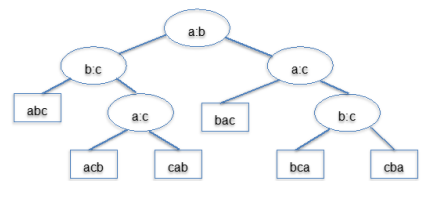
\includegraphics[width=0.7\linewidth]{dec_tree.png}
    \caption{Albero con 3 elementi}
    \label{fig:dec_tree}
\end{figure}

\noindent Passando ad un livello più generale è vero che:
\begin{itemize}
    \item Un array lungo $n$ ha $n!$ possibili ordinamenti
    \item Un albero alto $h$ ha al massimo $2^h$ foglie
\end{itemize}

\noindent $h$ deve essere tale che $2^h\geq n!\Rightarrow h\geq \log n!=\Theta(n\log n)$, quindi il costo minimo di un algoritmo basato sugli ordinamenti è $\Omega(n\log n)$.

\newpage

\paragraph{Mergesort} $\ $\newline

\noindent Questo algoritmo è basato sulla tecnica \textit{divide et impera}, ossia divide il problema in sottoproblemi e li risolve ricorsivamente (ogni chiamata riceve metà dell'array ed ordina i sottoarray):

\begin{algorithm}[ht]
\caption{Mergesort}
\begin{algorithmic}
\State Mer\_sort(A,index,index2):

    \If{index$<$index2}

        \State m=$\frac{index+index2}{2}$
        \State Mer\_sort(A,index,m)
        \State Mer\_sort(A,m+1,index2)
        \State Fondi(A,index,m,index2)

    \EndIf

\State

\State Fondi(A,index,m,index2): \Comment{Combina i 2 sottoarray in uno}

    \State i,j=index,m+1

    \State B=[]

    \While{$(i\leq \text{m})\And(j\leq\text{index2})$}

        \If{A[i]$\leq$A[j]}

            \State B.append(A[i])
            \State i++

        \Else

            \State B.append(A[j])
            \State j++        

        \EndIf

    \EndWhile

    \While{i$\leq$m}

        \State B.append(A[i])
        \State i++

    \EndWhile

    \While{j$\leq$index2}

        \State B.append(A[j])
        \State j++

    \EndWhile

    \For{$i\in[0,\text{len}(B)-1]$}

        \State A[index+i]=B[i]

    \EndFor

\end{algorithmic}
\end{algorithm}

\newpage

\noindent La funzione Fondi ha costo $\Theta(n)$ dato che tutti i cicli scorrono al più l'intero array, quindi $O(n)+O(n)+O(n)+\Theta(n)$, la funzione principale si può esprimere con l'equazione di ricorrenza:
\begin{equation}
    \nonumber
    \begin{split}
        T(n)&=2T(\frac{n}{2})+\Theta(n)\\
        T(1)&=\Theta(1)
    \end{split}
\end{equation}\newline

\noindent Che una volta risolta diventa $\Theta(n\log n)$.

\subparagraph{Merge-Insertion} $\ $\newline

\noindent Quando la dimensione dei sottoproblemi diventa abbastanza piccola l'Insertion Sort risulta più veloce del Mergesort, combinandoli si ottiene:

\begin{algorithm}[ht]
\caption{Merge\_Insertion}
\begin{algorithmic}
\State MerIns\_sort(A,index,index2,k,dim):

    \If{dim$>$k}

        \State m=$\frac{index+index2}{2}$
        \State MerIns\_sort(A,index,m,k,m-index+1)
        \State MerIns\_sort(A,m+1,index2,k,index2-index)
        \State Fondi(A,index,m,index2)

    \Else

        \State Ins\_Sort(index,index2)

    \EndIf
\end{algorithmic}
\end{algorithm}

\noindent L'equazione è:
\begin{equation}
    \nonumber
    \begin{split}
        T(n)&=2T(\frac{n}{2})+\Theta(n)\\
        T(k)&=\Theta(k^2)
    \end{split}
\end{equation}\newline

\noindent Se $k=O(\log n)$ il costo dell'algoritmo diventa $\Theta(n\log n)$.

\newpage

\paragraph{Quicksort} $\ $\newline

\noindent Anche questo algoritmo sfrutta il \textit{divide et impera}, la differenza sta nell'uso di un \textit{pivot} per dividere in sottoarray:

\begin{algorithm}[ht]
\caption{Quicksort}
\begin{algorithmic}
\State Quick\_sort(A,index,index2):

    \If{index$<$index2}

        \State m=Partiziona(A,index,index2)
        \State Quick\_sort(A,index,m-1)
        \State Quick\_sort(A,m+1,index2)

    \EndIf

\State

\State Partiziona(A,index,index2): \Comment{"Crea" i sottoarray}

    \State pivot=A[index]\Comment{Come si sceglie il pivot non è importante}

    \State i=index+1

    \For{$j\in[1+\text{index,index2}+1]$}

        \If{A[j]$<$pivot}

            \State scambia A[i]e A[j]

            \State i++

        \EndIf

    \EndFor

\State scambia A[i-1] e A[index]

\State return i-1

\end{algorithmic}
\end{algorithm}

\noindent Si nota facilmente che Partiziona ha costo $\Theta(n)$, con questa informazione si può scrivere l'equazione di ricorrenza:
\begin{equation}
    \nonumber
    \begin{split}
        T(n)&=T(k)+T(n-k-1)+\Theta(n)\text{ con $0\leq k\leq n-1$}\\
        T(1)&=\Theta(1)
    \end{split}
\end{equation}

\noindent Valutando i 3 possibili casi ottengo i costi:
\begin{itemize}

    \item Migliore: Sottoproblemi sempre bilanciati 

    $$2T(\frac{n-1}{2})+\Theta(n)=\Theta(\log n)$$

    \item Peggiore: Un sottoproblema è sempre nullo

    $$T(n-1)+\Theta(n)=\Theta(n^2)$$

    \item Medio: Il pivot suddivide gli elementi con egual probabilità

    $$\frac{1}{n-1}\left[ \sum_{k=0}^{n-1}(T(k)-T(n-k))\right]+\Theta(n)=\Theta(n\log n)$$
    
\end{itemize}

\paragraph{Heapsort} $\ $\newline

\noindent Questo algoritmo trasforma l'array in un Max-\hyperref[heap]{Heap} e sfrutta le sue caratteristiche, ad ogni iterazione scambia la radice con l'ultima foglia e risistema l'heap escludendo ad ogni iterazione l'ultima foglia:

\begin{algorithm}[ht]
\caption{Heapsort}
\begin{algorithmic}
\State Heap\_sort(A):

    \State Trasforma A in heap \Comment{$O(n\log n)$}

    \For{$x\in[\text{len}(A)-1,1]$} 

        \State Scambia A[0] e A[x]

        \State Heapify(A,0,x)

    \EndFor

\State

\State Heapify(A,i,size): \Comment{Aggiusta l'heap}

    \State l,r,max$=2i+1,2i+2,i$

    \If{(l$<$size)$\And$(A[l]$>$A[i])}

        \State max = l

    \EndIf

    \If{(r$\leq$size)$\And$(A[r]$>$A[max])}

        \State max = r

    \EndIf

    \If{max!=i}

        \State Scambia A[max] e A[i]

        \State Heapify(A,max,size)

    \EndIf

\end{algorithmic}
\end{algorithm}

\noindent Il costo totale è $T(n)=O(n)+O((n-1)\log n)=O(n\log n)$

\newpage

\subsubsection{Lineari}

I 2 algoritmi che verranno presi in considerazione hanno un costo lineare perché non sono basati su confronti.\newline

\paragraph{Counting Sort} $\ $\newline

\noindent Ipotizzando che l'array contenga solamente numeri interi compresi in un certo range $[0,k]$, creo un array ausiliario di lunghezza $k$ in cui conto le occorrenze di ogni numero e vado poi a sovrascrivere l'array originale:

\begin{algorithm}[ht]
\caption{Counting Sort}
\begin{algorithmic}
\State Count\_sort(A):

    \State C=Array di lunghezza max(A)+1

    \For{$i\in[0,\text{len}(A)-1]$} 

        \State C[A[i]]++

    \EndFor

    \State j=0

    \For{$i\in[0,\text{max}(A)]$} 

        \While{C[i]$>0$}

            \State A[j]=i
            \State j++
            \State C[i]$--$

        \EndWhile

    \EndFor

\end{algorithmic}
\end{algorithm}

\noindent Il costo è dato dalla somma dei due cicli $\Theta(n+k)$, se $k=O(n)\Rightarrow \Theta(n)$.\newline

\noindent Una cosa da tenere in considerazione è la dimensione dell'array ausiliario, infatti in casi come $A=\{4,6,1,2,55555\}$ $C$ occuperà inutilmente una grande quantità di memoria.\newline

\newpage

\subparagraph{Con dati satellite} $\ $\newline

\noindent Dato che l'array originale viene sovrascritto bisogna implementare delle modifiche per preservare eventuali dati satellite:

\begin{algorithm}[ht]
\caption{Counting Sort con dati satellite}
\begin{algorithmic}
\State Count\_sort2.0(A):

    \State C=Array di lunghezza max(A)$+1$
    \State B=Array di lunghezza len(A)

    \For{$i\in[0,\text{len}(A)-1]$} 

        \State C[A[i]]++

    \EndFor

    \For{$i\in[1,\text{max}(A)]$} 

        \State C[i]+=C[i-1]

    \EndFor

    \For{$i\in[\text{len}(A),-1]$} 

        \State B[C[A[j]]]=A[j]
        \State C[A[j]]$--$

    \EndFor

\State return B

\end{algorithmic}
\end{algorithm}

\vspace{-15pt}

\paragraph{Bucket Sort} $\ $\newline

\noindent In questo caso presumo che gli elementi siano equamente distribuiti nell'intervallo $[1,k]$, divido l'intervallo in sottointervalli detti \textit{bucket} di ampiezza uguale che verranno ordinati con un altro algoritmo e ricombinati alla fine:

\begin{algorithm}[ht]
\caption{Bucket Sort}
\begin{algorithmic}
\State Buck\_sort(A):

    \State Crea i bucket in base a max(A) \Comment{Bucket=\hyperref[lista]{Lista}}

    \For{$i\in[0,\text{len}(A)-1]$} 

        \State Inserisci A[i] nell'apposito bucket 

    \EndFor

    \For{$i\in[0,\text{len}(A)-1]$} 

        \State Ordina l'i-esimo bucket

    \EndFor

    \State Combina i bucket (seguendo l'ordine $B_1,B_2,\ldots$) in un'unica lista
    \State Copia la lista in A

\end{algorithmic}
\end{algorithm}

\vspace{-5pt}

\noindent Il costo dipende da:
\begin{itemize}
    \item Distribuzione dei numeri nei bucket
    \item Numero e lunghezza dei bucket
    \item Algoritmo di ordinamento usato\newline
\end{itemize}

\vspace{-5pt}

\noindent In ogni caso il costo medio è $O(n+k+\frac{n^2}{k})$ che diventa lineare se $k=n$.

\section{Strutture dati}

Una struttura dati memorizza e manipola insiemi dinamici di dati varianti nel tempo, ogni elemento (o nodo) può poi essere composto da molteplici dati elementari, comunemente sono composti da:
\begin{itemize}
    \item Chiave: usata per distinguere gli elementi
    \item Dati satellite: altri dati non usati direttamente\newline
\end{itemize}

\noindent Le tipiche operazioni che si possono svolgere sono:
\begin{itemize}
    \item Ricerca di un elemento
    \item Ricerca del minimo/massimo
    \item Ricerca dell'elemento precedente/successivo
    \item Inserimento di un nuovo elemento
    \item Cancellazione di un elemento
\end{itemize}

\subsection{Array}

Un array ha le seguenti caratteristiche:
\begin{itemize}
    \item Ogni elemento è omogeneo
    \item Ha l'accesso casuale
    \item Ha dimensione fissa
\end{itemize}


\begin{table}[ht]
    \centering
    \begin{tabular}{c|c|c|c|c|c}
        Array & Ricerca & Min/Max & Prec/Succ & Inserimento & Cancellazione\\
        \hline
        generico & $O(n)$ & $\Theta(n)$ & $\Theta(n)$ & $\Theta(1)$ & $\Theta(1)$\\
        \hline
        ordinato & $O(\log n)$ & $\Theta(1)$ & $\Theta(1)$ & $O(n)$ & $O(n)$\\
    \end{tabular}
    \label{tab:costo_array}
\end{table}

\newpage

\subsection{Lista}\label{lista}

\textbf{Definizione} Un puntatore è una variabile che contiene l'indirizzo in memoria di un'altra variabile.\newline

\noindent\textbf{Definizione} Una lista è una struttura dati che organizza i suoi elementi in sequenza, le sue proprietà sono:
\begin{itemize}
    \item L'accesso è solo sequenziale
    \item L'accesso avviene all'inizio o alla fine della lista
\end{itemize}

\subsubsection{Semplice}

In questo caso un nodo conterrà un puntatore all'elemento successivo:

\begin{figure}[H]
    \centering
    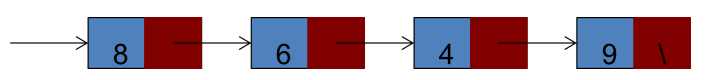
\includegraphics[width=0.7\linewidth]{lista.png}
    \label{fig:lista}
\end{figure}

\subsubsection{Doppia}

Per diminuire il costo della cancellazione si può inserire nel nodo anche un puntatore all'elemento precedente:

\begin{figure}[ht]
    \centering
    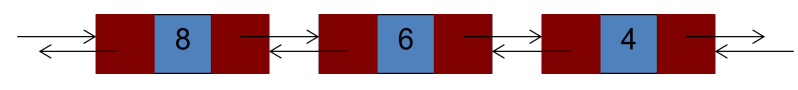
\includegraphics[width=0.7\linewidth]{lista2.png}
    \label{fig:lista2}
\end{figure}

\begin{table}[ht]
    \centering
    \begin{tabular}{c|c|c|c|c|c}
        Lista & Ricerca & Min/Max & Prec/Succ & Inserimento & Cancellazione\\
        \hline
        semplice & $O(n)$ & $\Theta(n)$ & $\Theta(n)$ & $\Theta(1)$ & $O(n)$\\
        \hline
        doppia & $O(n)$ & $\Theta(n)$ & $\Theta(n)$ & $\Theta(1)$ & $\Theta(1)$\\
    \end{tabular}
    \label{tab:costo_lista}
\end{table}

\paragraph{Circolare} $\ $\newline

\noindent Un'implementazione particolare è quella in cui l'ultimo elemento viene fatto puntare al primo creando così un cerchio:

\begin{figure}[ht]
    \centering
    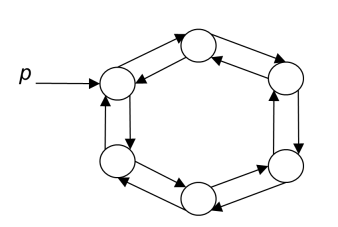
\includegraphics[width=0.4\linewidth]{lista3.png}
    \label{fig:lista3}
\end{figure}

\newpage

\subsection{Coda}

\textbf{Definizione} La coda è una struttura con comportamento \textit{FIFO}, ossia gli elementi vengono prelevati (operazione Dequeue) nell'ordine con cui sono stati inseriti (operazione Enqueue), ha una struttura:

\begin{figure}[ht]
    \centering
    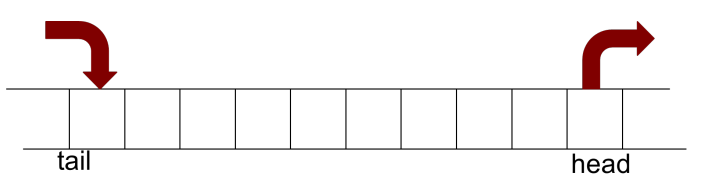
\includegraphics[width=0.7\linewidth]{coda.png}
    \label{fig:coda}
\end{figure}

\begin{table}[ht]
    \centering
    \begin{tabular}{c|c|c}
        Coda & Enqueue & Dequeue\\
        \hline
         & $\Theta(1)$ & $\Theta(1)$\\
    \end{tabular}
    \label{tab:costo_coda}
\end{table}

\subsubsection{Con priorità}

Una variante è quella in cui la posizione di un elemento non dipende dall'istante di inserimento ma da un altro valore detto di priorità (contenuto nel nodo). Un potenziale problema di questa variante è quello della \textit{starvation} in cui un elemento non verrà mai estratto se viene scavalcato in continuazione da nuovi elementi con più priorità.

\subsection{Pila}

\textbf{Definizione} La pila è una struttura con comportamento \textit{LIFO}, ossia gli elementi vengono prelevati (operazione Pop) nell'ordine inverso con cui sono stati inseriti (operazione Push), ha una struttura:

\begin{figure}[ht]
\begin{minipage}[t]{0.49\textwidth}
\begin{figure}[H]
    \centering
    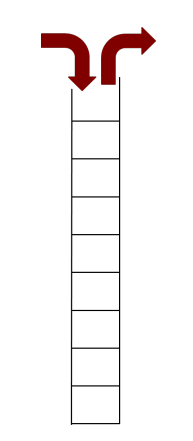
\includegraphics[width=0.4\linewidth]{pila.png}
    \label{fig:pila}
\end{figure}
\end{minipage}
\begin{minipage}[t]{0.49\textwidth}
\begin{table}[H]
    \centering
    \begin{tabular}{c|c|c}
        Pila & Pop & Push\\
        \hline
         & $\Theta(1)$ & $\Theta(1)$\\
    \end{tabular}
    \label{tab:costo_pila}
\end{table}
\end{minipage}
\end{figure}

\subsection{Grafo}

\textbf{Definizione} Un grafo è una coppia di insiemi $(V,E)$ tali che:
\begin{itemize}
    \item $V$ è un insieme di nodi
    \item $E\subseteq V\times V$ è un insieme di archi tra i nodi\newline
\end{itemize}

\begin{figure}[ht]
    \centering
    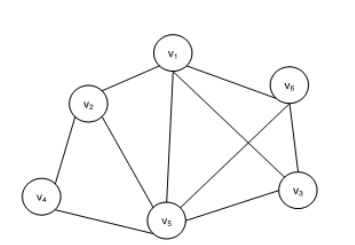
\includegraphics[width=0.6\linewidth]{grafo.png}
    \caption{Esempio di Grafo}
    \label{fig:grafo}
\end{figure}

\noindent\textbf{Definizione} Un cammino è una sequenza di nodi $(v_1,v_2,\ldots,v_k)\ |\ \forall\ i\ \ 1\leq i\leq k-1\ \ \exists(v_i,v_{i+1})\in E $.\newline 

\noindent\textbf{Definizione} Un ciclo è un cammino che inizia e finisce sullo stesso nodo.\newline

\noindent\textbf{Definizione} Un grafo è detto aciclico se non contiene cicli.\newline

\noindent\textbf{Definizione} Un grafo è detto connesso se esiste un cammino tra ogni coppia di nodi.

\newpage

\subsection{Albero}

\textbf{Definizione} Un albero è un grafo connesso e aciclico.\newline

\noindent\textbf{Definizione} Un albero radicato è un albero in cui è presente un elemento chiamato \textit{radice}, si rappresenta graficamente mettendo la radice in alto e rappresentando i cammini verso il basso organizzandoli a livelli:

\begin{figure}[ht]
    \centering
    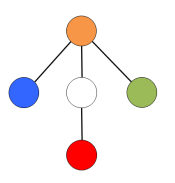
\includegraphics[width=0.3\linewidth]{albero.png}
    \caption{Esempio di albero}
    \label{fig:albero}
\end{figure}

\noindent\textbf{Definizione} Il padre di un nodo $x$ è il nodo che si incontra prima di lui nel cammino dalla radice, viceversa si dice figlio di $x$.\newline

\noindent\textbf{Definizione} I nodi con lo stesso padre si chiamano fratelli.\newline

\noindent\textbf{Definizione} L'antenato di un nodo $x$ è qualsiasi nodo incontrato sul cammino per raggiungere $x$.\newline

\noindent\textbf{Definizione} I discendenti di un nodo $x$ sono tutti i nodi che hanno come antenato $x$.\newline

\noindent\textbf{Definizione} Un nodo senza figli si chiama foglia.\newline

\noindent\textbf{Definizione} L'altezza di un albero radicato è la lunghezza del cammino più lungo dalla radice ad una foglia.\newline

\noindent\textbf{Definizione} Un albero radicato è detto ordinato se tutti i figli di ogni nodo hanno un qualche ordine.\newline

\newpage

\subsubsection{Binario}

\noindent\textbf{Definizione} Un albero binario è un albero radicato e ordinato in cui ogni nodo ha al massimo 2 figli definiti sinistro e destro.\newline

\noindent\textbf{Definizione} Un albero binario è detto completo se ogni livello ha il massimo numero possibile di nodi.\newline

\noindent\textbf{Definizione} Un albero binario è detto quasi completo se tutti i livelli sono pieni ma l'ultimo solo in parte (da sinistra a destra).\newline

\paragraph{Rappresentazione in memoria} $\ $\newline

\noindent Ci sono 3 possibilità per memorizzare un albero binario:
\begin{enumerate}
    \item \textbf{Con record e puntatori}

    Un nodo è formato dal campo chiave e 2 puntatori ai figli.

    \item \textbf{Posizionale} 

    Si usa un array con la radice in posizione 0, i figli di un nodo all'indice $i$ saranno in posizione $2i,2i-1$.

    \item \textbf{Vettore dei padri}

    Si usa un vettore in cui l'indice $i$ corrisponde al nodo $i$ e contiene l'indice del padre di $i$.
    
\end{enumerate}

\paragraph{Visita dei nodi}$\ $\newline

\noindent Accedere a tutti i nodi risulta leggermente più complicato delle altre strutture, i possibili modi per visitare tutti i nodi sono 3:
\begin{enumerate}
    \item \textbf{Preorder}

    Prima visito il nodo e poi i sottoalberi.
    
    \item \textbf{Inorder}

    Visito il sottoalbero sinistro, il nodo e poi il sottoalbero destro.
    
    \item \textbf{Postorder}

    Il nodo è visitato dopo le visite ai sottoalberi.
    
\end{enumerate}

\noindent Nel caso in cui si usino i puntatori l'opzione migliore è usare una funzione ricorsiva, indipendentemente dal tipo di visita il costo è $\Theta(n)$.

\subsubsection{Heap}\label{heap}

\textbf{Definizione} Un Max-Heap è un albero binario completo (o quasi) con la seguente caratteristica:\textit{ ogni chiave di un nodo è più grande delle chiavi dei suoi discendenti}, ovviamente esiste anche il Min-Heap con la caratteristica opposta.\newline

\noindent Data la loro struttura risulta evidente che trovare il massimo/minimo ha costo $\Theta(1)$ essendo esso la radice.

\subsubsection{ABR}

\textbf{Definizione} Un albero binario di ricerca è un albero binario con la seguente caratteristica:

\begin{figure}[ht]
    \centering
    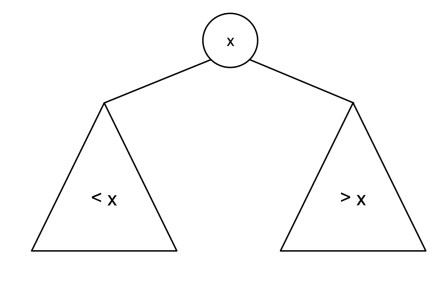
\includegraphics[width=0.6\linewidth]{abr.png}
    \caption{Struttura ABR}
    \label{fig:abr}
\end{figure}

\noindent Il costo delle operazioni dipende dal bilanciamento dell'albero:
\begin{itemize}
    \item Caso peggiore:

    Se l'albero è degenere (graficamente si immagini una diagonale) potrebbe essere necessario scorrerlo interamente, quindi $O(n)$.

    \item Caso migliore:

    Se l'albero è completo diventa simile ad una ricerca binaria, il costo è $\Omega(\log n)$.    
    
\end{itemize}

\newpage

\subsubsection{Rosso-nero}

\textbf{Definizione} Una foglia fittizia è una foglia senza valore che viene eventualmente aggiunta ad un nodo per fargli avere 2 figli.\newline

\noindent\textbf{Definizione} Un albero-RB è un ABR con le seguenti caratteristiche:
\begin{itemize}
    \item I nodi hanno un campo aggiuntivo che contiene il loro colore (Rosso o nero)
    \item Un nodo rosso ha entrambi i figli neri
    \item Ogni foglia fittizia è nera
    \item La radice è nera
    \item Ogni cammino da un nodo ad una sua foglia discendente contiene lo stesso numero di nodi neri, il numero di nodi neri si indica con \textit{b-altezza}
\end{itemize}

\begin{figure}[ht]
    \centering
    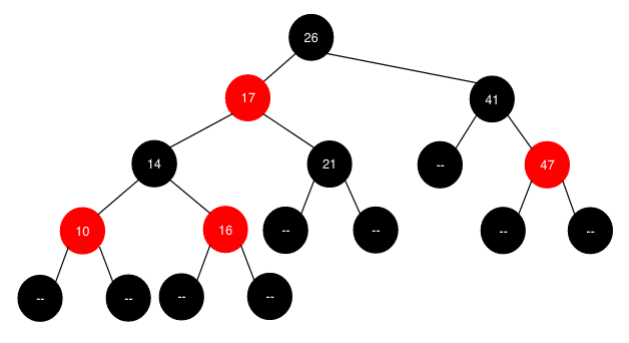
\includegraphics[width=\linewidth]{arb.png}
    \caption{Esempio di albero RB}
    \label{fig:arb}
\end{figure}

\noindent Queste caratteristiche permettono di avere un albero la cui altezza è sempre:

$$h\leq2\log(n+1)\text{ con $n$ nodi interni}$$\newline

\newpage

\paragraph{Rotazione} $\ $\newline

\noindent Questo albero ha una particolare operazione detta \textit{rotazione} (a DX o SX) che gli permette di mantenere le caratteristiche dopo un inserimento o cancellazione in $O(\log n)$.\newline

\noindent Nello specifico la rotazione a SX di un nodo $x$ consiste in:
\begin{enumerate}
    \item Il sottoalbero sinistro del figlio destro di $x$ diventa il sottoalbero destro di $x$
    \item $x$ diventa il figlio sinistro del suo figlio destro\newline
\end{enumerate}

\begin{figure}[ht]
    \centering
    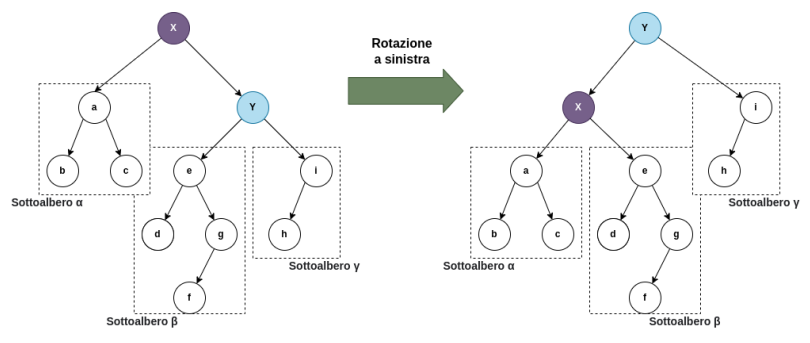
\includegraphics[width=\linewidth]{arb2.png}
    \caption{Esempio di rotazione a SX}
    \label{fig:arb2}
\end{figure}

\subsection{Dizionario}

\textbf{Definizione} Un dizionario è una struttura dati che permette di gestire un insieme dinamico di dati (normalmente ordinato) con 3 sole operazioni:
\begin{itemize}
    \item Inserisci
    \item Cancella
    \item Cerca\newline
\end{itemize}

\noindent Da qui in poi:
\begin{itemize}
    \item $U=$ insieme dei valori delle chiavi
    \item $n=$ numero di elementi da memorizzare
    \item $m=$ numero di posizioni disponibili
\end{itemize}

\subsubsection{Indirizzamento diretto}

Ipotizzando $n\leq|U|=m$ basta un array con $m$ posizioni che permette di avere le operazioni con costo $\Theta(1)$.\newline

\noindent Nella realtà però non è un metodo utilizzabile perché:
\begin{enumerate}
    \item $U$ potrebbe essere enorme
    \item Le chiavi effettivamente usate potrebbe essere poche e ciò porta ad uno spreco di memoria\newline
\end{enumerate}

\subsubsection{Hash}

Per risolvere il problema del metodo precedente viene fatto uso di una funzione detta \textit{hash} che fornisce la posizione dove inserire l'elemento in base alla sua chiave.\newline

\noindent Le 3 funzioni più comuni sono:
\begin{itemize}
    \item Scansione lineare:

    $$h(k,i)=(h'(k)+i)\mod m\text{ 
 con } i\in[0,m-1]$$

    \item Scansione quadratica:

    $$h(k,i)=(h'(k)+c_1i+c_2i^2)\mod m\text{ 
 con } i\in[0,m-1]$$

    \item Hashing doppio:

    $$h(k,i)=(h_1(k)+h_2(k)i)\mod m\text{ 
 con } i\in[0,m-1]$$
    
\end{itemize}

\noindent Anche questo metodo ha un problema, bisogna trovare una funzione per cui un'eventuale collisione (la funzione dà una posizione già occupata) avvenga con la probabilità più bassa possibile.

\paragraph{Risoluzione delle collisioni} $\ $\newline

\noindent Ci sono 2 metodi per affrontare il problema:
\begin{enumerate}
    \item Liste di trabocco

    Essenzialmente viene associata una lista ad ogni possibile output della funzione, mediamente il costo di ricerca/cancellazione diventa $\Theta(1+\frac{n}{m})$.

    \item Indirizzamento aperto

    Nella funzione si tiene conto anche del numero di collisioni incontrate $h(k,0),h(k,1),\ldots$, bisogna però gestire la cancellazione che lasciando una casella vuota può portare a risultati errati nella ricerca.
    
\end{enumerate}

\end{document}
